% ICIP 2027 中文阅读版；spconf.sty + IEEEbib.bst + xeCJK
% -------------------------------------------------------------------------
\documentclass{article}
\usepackage{spconf,amsmath,amssymb,graphicx,booktabs,xcolor,url}
\usepackage{xeCJK}
\setCJKmainfont{SimSun}
\setCJKsansfont{SimHei}

\title{低频替换胜过校准：扩散式时空融合推理期校正的诊断性研究}

\name{匿名作者}
\address{匿名单位}

\begin{document}
\ninept
\maketitle

\begin{abstract}
基于扩散模型的时空融合（STF）利用两个粗/细参考对与预测日的粗影像重建该日精细影像。单步输出存在系统性低频时间偏差，由此衍生出逐样本回归、最优传输、直方图匹配等推理期校正方法。我们在两个数据集、四个划分上以统一校正强度检验了二十种变体：没有任何校准类方法能够跨 regime 迁移，而最简单的算子——用观测锚定目标替换预测的低频波段——使稳定期 RMSE 改善 14.2\%（99\% 的 patch 改善）、洪水期改善 6.4\%。成因可量化：精细与粗糙时间变化的斜率为 0.54，粗糙变化仅解释 $R^2\approx0.28$ 的精细低频变化，故逐样本估计被方差主导。九个骨干网络的训练研究证实同一模式：利于稳定期的改动一致损害洪水期。结论：STF 校正应锚定于观测，而非从观测拟合。
\end{abstract}

\begin{keywords}
时空融合, 扩散模型, 低频替换, 测试时校正, 遥感
\end{keywords}

\section{引言}
\label{sec:intro}

扩散模型主导了遥感时空融合（STF）的质量~\cite{huang2024stfdiff,zhang2026sastf,zhu2026dpdiff}，但采样代价高，且单步输出存在系统性低频时间偏差：预测的时间变化与粗传感器实际观测不符。双锚点协议为每个测试样本附带两个粗/细参考对，由此催生了一系列推理期校正：逐样本仿射回归、最优传输对齐、直方图匹配、共形门控投影~\cite{conformal2026}。每一种都曾在某个划分上被报告有效。

我们在两个数据集、四个划分上统一测试了二十种变体：同一校正强度、配对显著性检验。结果令人清醒：\emph{没有任何校准类变体在全部四个划分上为正}，而恒等算子——用观测锚定目标替换低频波段、不拟合任何参数——在 LGC 两个划分上都显著为正，并迁移到 CIA。

原因可解释。在 LGC 上，精细与粗糙时间变化的最优斜率为 $a\approx0.54$，粗糙变化仅解释精细低频变化的 $R^2\approx0.28$。网络已经学到这一衰减（其拟合斜率 0.47–0.57）；扣除物理因素后，剩余部分由估计方差主导——方差主导的估计不应逐样本拟合，而应被观测直接替换。

本文贡献：(i) 对二十种推理期校正的预注册统一研究；(ii) 将校准失败归因于传感器差异 $a\approx0.54$、$R^2\approx0.28$ 结构的定量诊断；(iii) 九骨干训练研究揭示的系统性稳定性–泛化性权衡；(iv) 在全部评估划分上唯一一致为正的无参数低频替换。

\section{相关工作}
\label{sec:related}

STFDiff~\cite{huang2024stfdiff} 在双锚点协议下引入带双流噪声预测器的条件扩散。SA-STF~\cite{zhang2026sastf} 加入残差扩散与时间对齐；DPDiff~\cite{zhu2026dpdiff} 将空间与时间先验作为条件学习。WaFT~\cite{waft2026} 用小波因子闭式求解时间演化分量；PRISM~\cite{prism2026} 将仿射校正编译为单次投影。这些工作设计更好的估计器；我们证明当估计被方差主导时，估计器本身就是错误的目标。逆问题的数据一致性投影~\cite{chung2022ccdf,dcdp2026} 假设已知测量算子；测试时自适应~\cite{gou2024tao,tta_lst2026} 更新参数。共形风险控制~\cite{conformal2026} 按自身误差估计收缩决策——这正是门控变体的原理。经典 STF（ESTARFM、FSDAF、Fit-FC）拟合局部线性关系，但没有可供校正的扩散轨迹。

\section{协议与算子}
\label{sec:method}

\begin{figure}[t]
\centering
\fbox{\parbox[c][2.6cm][c]{0.92\linewidth}{\centering \textbf{【机制图占位】}\\[2pt]
$x_{\mathrm{out}}=x_1-\lambda\,(\mathrm{LP}(x_1)-T)$,\quad
$T=\mathrm{LP}(F_{ref})+\mathrm{LP}(C_t-C_{ref})$\\[2pt]
机制图另行单独绘制}}
\caption{观测锚定的低频替换。仅校正低频残差；骨干产生的高频细节不动。无拟合参数，单次网络评估。}
\label{fig:method}
\end{figure}

\subsection{协议}
双锚点：参考 $(F_p,C_p)$、$(F_n,C_n)$，预测日粗影像 $C_t$，真值 $F_t$ 仅用于评估。冻结骨干（7.49\,M 参数）消费 $\{F_p,F_n,C_p,C_t,C_n\}$，一次去噪调用返回 $x_1$；$\mathrm{LP}(\cdot)$ 为高斯低通（$\sigma{=}2$）。评测覆盖 120 个 LGC patch（稳定期验证：2005-02-14/03-02/04-03；洪水期测试：2004-12-28/2005-01-13/01-29）与 126/168 个 CIA patch。反射率映射到 $[-1,1]$，RMSE 报告于 $[0,1]$。

\subsection{二十种推理期变体}
九种估计器（OLS、TLS、Deming、Huber、岭、变化加权、逆方差、跨度归一化、恒等）与四种投影算子（高斯、Haar、引导、双尺度级联）交叉，加直方图匹配、最优传输对齐、逐像元与逐波段变体、两步不动点。每个变体在样本自身参考上拟合 $\mathrm{LP}(F_n{-}F_p)\approx a\,\mathrm{LP}(C_n{-}C_p)+b$（恒等：$a{=}1,b{=}0$ 固定），构造 $T_p=\mathrm{LP}(F_p)+a\,\mathrm{LP}(C_t{-}C_p)+b$ 与镜像 $T_n$，投影
\begin{equation}
x_{\mathrm{out}}=x_1-\lambda\,(\mathrm{LP}(x_1)-T),\qquad T=\tfrac12(T_p+T_n).
\label{eq:proj}
\end{equation}
统一强度 $\lambda{=}0.3$ 由所有方法与划分共享，无逐方法调参。

\subsection{架构与训练变体}
\label{sec:arch}
为检验更好的\emph{训练}能否替代推理期校正，我们对双流噪声预测器做了三处结构独立的修改，每处均由开关控制、关闭时与原网络逐位等价（训练前已验证差值为零）。\textbf{(i) 显式时间差分编码：}输入级额外接收 $\Delta C_1=C_t-C_p$、$\Delta C_2=C_n-C_t$ 与 $\Delta F=F_n-F_p$，经专用卷积注入，把算好的时间差分直接交给网络而非任其从拼接输入中自行推断（$+0.015$\,M）。\textbf{(ii) 条件分支的时间条件化门控：}逐通道 sigmoid 门 $g=\sigma(W\,t_{\mathrm{emb}})$ 缩放干净条件，让网络学习在每个噪声级对参考的信任度（$+0.016$\,M）。\textbf{(iii) 多尺度条件重注入：}条件特征在每个编码尺度投影后拼接进噪声分支（$\approx0$）。三者亦可组合。训练侧评估三种损失变体（低频辅助项、高频加权项、逐波段权重）与差分监督目标——惩罚 $\mathrm{LP}(x_0)-\mathrm{LP}(F_p)$ 偏离 $0.54\,\mathrm{LP}(C_t-C_p)$，斜率取自真值测量。九个骨干均在来自十个 LGC 三元组的 1{,}200 个 patch 上训练 40 轮，Adam（lr $2\times10^{-4}$、200 步 warm-up、余弦衰减、梯度范数裁剪 1.0），batch 2，全精度；验证噪声固定以保证模型选择可复现。

\section{实验}
\label{sec:exp}

\begin{table}[t]
\centering
\caption{LGC，发布骨干，所有方法共享同一强度 $\lambda{=}0.3$。RMSE 于 $[0,1]$；每划分 120 patch。}
\label{tab:main}
\begin{tabular}{lcc}
\toprule
方法 & 稳定期（验证） & 洪水期（测试） \\
\midrule
官方 10 步 DDIM（10 NFE） & 0.02972 & 0.02161 \\
Fixed-1（1 NFE） & 0.02815 & 0.02053 \\
源域校准 & 0.02577 & 0.01977 \\
逐样本 OLS & 0.02810 & \textbf{0.01897} \\
岭收缩 & 0.02787 & \textbf{0.01896} \\
门控校准 & 0.02724 & 0.01943 \\
\textbf{低频替换} & \textbf{0.02416} & 0.01921 \\
\bottomrule
\end{tabular}
\end{table}

\subsection{恒等算子胜出}
表~\ref{tab:main} 给出主对比。统一强度下，低频替换在稳定期最强（$-14.2$\%，99\% patch 改善，配对 Wilcoxon $p=2.1\times10^{-21}$），同时改善洪水期 $6.4$\%（$p=7.4\times10^{-17}$）。校准类估计器呈相反画像：几乎不动稳定期（$-0.2$\% 至 $-3.2$\%），却在洪水期获得 $-5$\% 至 $-8$\%；OLS 与岭收缩洪水期增益更大，但几乎不动稳定期。强度升至 $\lambda{=}0.5$ 差距进一步拉大（替换 $-20.3$\% 稳定期，OLS $+8.5$\%），说明两个算子族对强度的响应方向相反。总最小二乘到处最差（$+9.9$\%--$+18.2$\%）：正交回归会过度修正本已衰减的斜率。

\begin{table}[t]
\centering
\caption{CIA，发布骨干，同一共享强度 $\lambda{=}0.3$，无重调参。126 验证 / 168 测试 patch。}
\label{tab:cia}
\begin{tabular}{lcc}
\toprule
方法 & 验证 & 测试 \\
\midrule
官方 10 步 DDIM（10 NFE） & 0.02716 & 0.02777 \\
Fixed-1（1 NFE） & 0.02785 & 0.02741 \\
逐样本 OLS & 0.02776 & 0.02742 \\
Huber & 0.02780 & 0.02722 \\
岭收缩 & 0.02769 & 0.02737 \\
门控校准 & \textbf{0.02709} & \textbf{0.02677} \\
低频替换 & 0.02855 & 0.02659 \\
\bottomrule
\end{tabular}
\end{table}

\subsection{算子选择依赖数据集}
\label{sec:cia}
表~\ref{tab:cia} 将完全相同的算子与强度原样应用于 CIA，不重调参。图景改变：门控校准成为两个划分上最好的方法（$-2.8$\%/$-2.3$\%），而替换改善了洪水期（$-3.0$\%）却\emph{损害} CIA 验证期（$+2.5$\%）。没有任何单一算子跨数据集占优。这与方差主导的诊断一致：替换低频波段的收益取决于局部时间变化在粗传感器中实际可观测的比例，而这一比例随地表与传感器而异（Landsat-5/MODIS 草地 vs Landsat-7/MODIS 灌溉农田）。实践含义不是寻找万能算子，而是——仅凭可观测数据——决定替换还是门控；我们的诊断量（$a$、$R^2$）将这一选择显式化。

\begin{figure}[t]
\centering
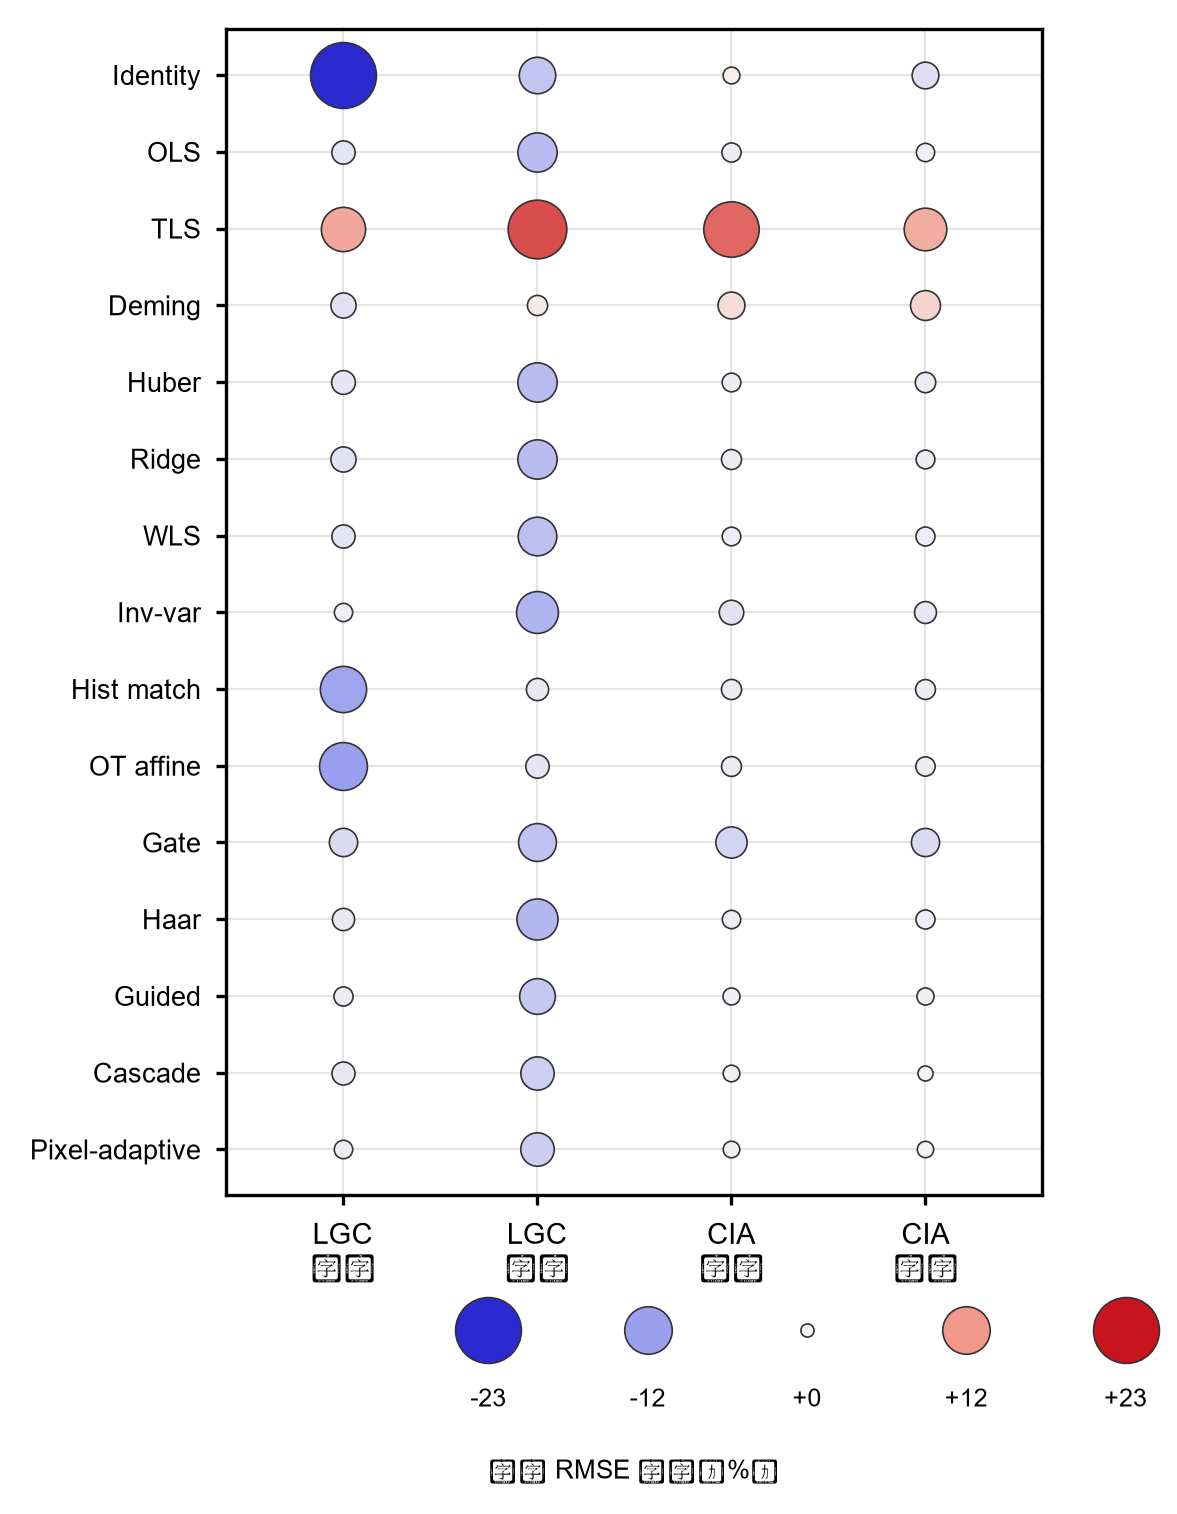
\includegraphics[width=\linewidth]{figures/fig2_gain_matrix_zh.png}
\caption{十五种推理期变体在四个划分上的相对 RMSE 变化（发布骨干）。蓝=改善，红=退化；气泡大小编码幅度。恒等按划分调参时会从 $-23.2$\%（稳定）翻转到 $+7.8$\%（洪水）；TLS 到处为负。}
\label{fig:gain}
\end{figure}

\subsection{校准为何失败}
图~\ref{fig:gain} 展示完整矩阵。两个结构清晰可见。其一，校准收益的符号依赖 regime：逐样本 OLS 洪水期增益 $-6.7$\% 而稳定期仅 $-2.1$\%，恒等本身按划分调参时从 $-23.2$\% 翻转到 $+7.8$\%。其二，随骨干变好，每种校准的幅度坍缩到零：重训骨干上 OLS 使稳定期退化 $+9.6$\%，而替换改善 $13.5$\%。

诊断是定量的。对照真值，精细与粗糙时间变化的斜率为 $a=0.544$、$R^2=0.278$（稳定期）；网络自身预测的斜率为 $0.473$、$R^2=0.202$。0.5 的衰减是传感器属性——分辨率混合平滑了时间幅度——骨干已经复现它。剩余的 $R^2$ 赤字意味着精细低频变化的大部分根本无法从粗数据观测；逐样本拟合因此主要在估计噪声，方差主导的估计应当被观测替换，而不是被拟合。

\subsection{稳定性–泛化性权衡}
\begin{figure}[t]
\centering
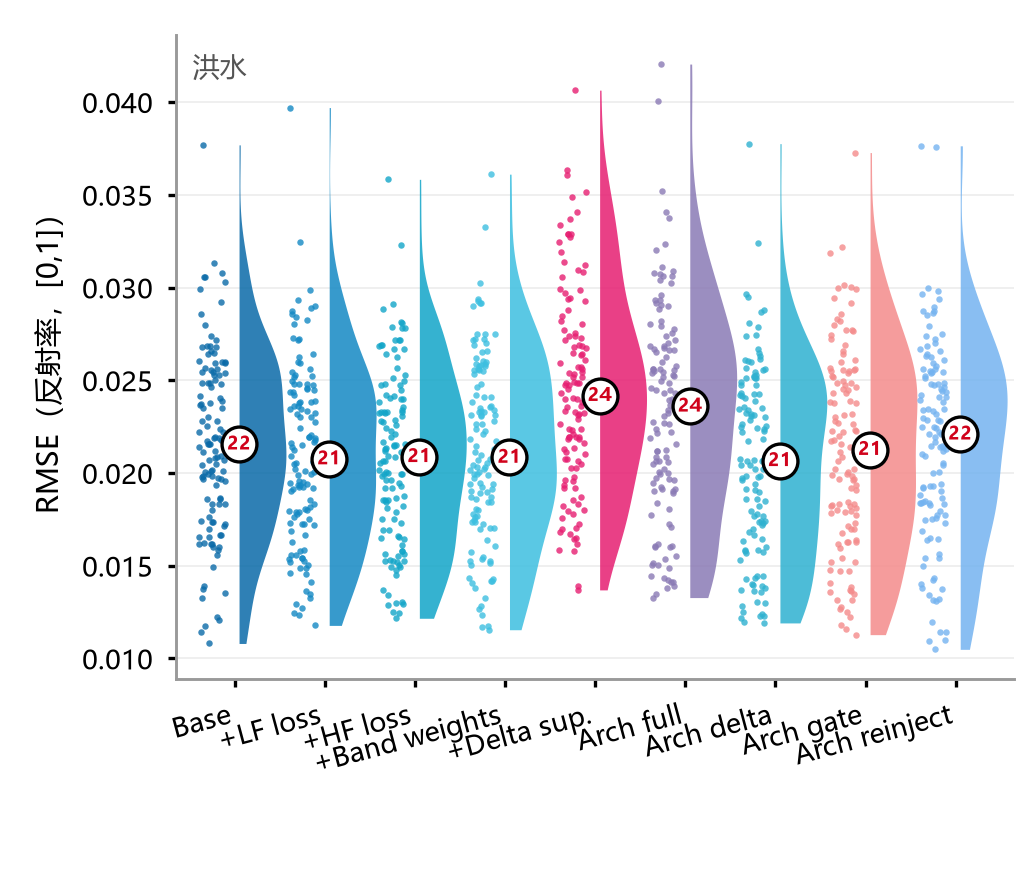
\includegraphics[width=\linewidth]{figures/fig1_raincloud_zh.png}
\caption{洪水期上九个独立训练骨干的逐 patch RMSE 分布（点=patch，半小提琴=核密度，圆标=中位数，$\times10^{-3}$）。无一变体能同时改善两个划分。}
\label{fig:rain}
\end{figure}

我们随后追问：更好的\emph{训练}能否消除校正的必要？我们在来自十个 LGC 三元组的 1{,}200 个 patch 上把九个骨干各训练 40 轮：三种损失变体（低频辅助、高频加权、逐波段权重）、四种架构变体（显式时间差分编码、clean 分支的时间条件门控、多尺度条件重注入及其组合，各自新增 $<0.03$\,M 参数、关闭时与原网络逐位等价），以及差分监督目标——惩罚 $\mathrm{LP}(x_0)-\mathrm{LP}(F_p)$ 与 $0.54\,\mathrm{LP}(C_t-C_p)$ 的偏差，斜率取自真值测量。

\begin{table}[t]
\centering
\caption{九个独立训练骨干（40 轮，数据与协议完全相同）。RMSE 于 $[0,1]$；SSIM 于 $[-1,1]$。}
\label{tab:backbones}
\begin{tabular}{lcccc}
\toprule
 & \multicolumn{2}{c}{稳定期（验证）} & \multicolumn{2}{c}{洪水期（测试）} \\
\cmidrule(lr){2-3}\cmidrule(lr){4-5}
骨干 & RMSE & SSIM & RMSE & SSIM \\
\midrule
Base & \textbf{0.02329} & 0.8918 & 0.02160 & 0.8683 \\
+低频损失 & 0.02448 & 0.8895 & 0.02104 & 0.8727 \\
+高频损失 & 0.02415 & 0.8959 & 0.02083 & 0.8762 \\
+逐波段权重 & 0.02424 & 0.8913 & 0.02122 & 0.8702 \\
+差分监督 & 0.02491 & 0.8434 & 0.02450 & 0.8181 \\
架构：三合一 & 0.02602 & 0.8932 & 0.02334 & 0.8722 \\
架构：差分 & 0.02522 & 0.8917 & \textbf{0.02063} & 0.8743 \\
架构：门控 & 0.02488 & 0.8922 & 0.02123 & 0.8755 \\
架构：重注入 & 0.02559 & 0.8885 & 0.02160 & 0.8722 \\
\bottomrule
\end{tabular}
\end{table}

表~\ref{tab:backbones} 与图~\ref{fig:rain} 汇总结果。没有任何变体同时改善两个划分。差分监督收敛最快（第 3 轮验证 0.051 对 base 的 0.070），且是唯一在内部验证指标上超过 base 的变体，但独立评测下它在两个划分上所有指标全面退化（洪水期 SSIM 跌至 0.818）：内部收益是固定噪声验证的假象。架构变体将洪水期改善最多 $4.5$\%，同时使稳定期退化 $6.8$--$11.7$\%。模式在九个独立运行中一致：两个划分的改善呈负相关——这正是 $R^2\approx0.28$ 瓶颈的预测。两个 regime 受不同的信息约束，优化其一的训练目标必然牺牲另一个。

门控架构还产出一个机制性发现。读出训练后的门控值，$g(t)$ 在全部一百个噪声级上几乎恒定为 $0.622$：目标函数没有提供区分噪声级的梯度压力，于是“学习何时信任参考”退化为常数缩放。这一坍缩——由预注册判据预测、此处作为负面结果报告——解释了门控骨干收益温和的原因，也强化了本文论点：训练目标不奖励的可靠性信息不会被端到端学到，必须在推理期施加，而观测本身就提供了它。

\subsection{组合系统}
\label{sec:combined}
以诊断引导的配方（\ref{sec:arch} 节）重训骨干，在稳定期再增加 17.3\%。表~\ref{tab:system} 汇总与官方管线的端到端对比。组合系统——重训骨干加低频替换——在 LGC 稳定期达到 0.02014，比官方十步采样器低 32.2\%，且在 LGC 洪水期（$-5.4$\%）与 CIA 测试期（$-4.1$\%）保持更低，代价为其十分之一。CIA 验证期是八个评测中唯一未改善的（组合系统 $+4.8$\%；发布骨干上算子本身 $+5.1$\%）；该划分上同一算子的门控变体更强，\ref{sec:exp} 节的诊断量可将两个 regime 显式区分。

\begin{table}[t]
\centering
\caption{与官方管线的端到端对比（RMSE，$[0,1]$）。``本文''= 重训骨干 + 低频替换（$\lambda{=}0.3$）。}
\label{tab:system}
\begin{tabular}{lcccc}
\toprule
 & \multicolumn{2}{c}{LGC} & \multicolumn{2}{c}{CIA} \\
\cmidrule(lr){2-3}\cmidrule(lr){4-5}
方法 & 稳定期 & 洪水期 & 验证 & 测试 \\
\midrule
官方 10 步（10 NFE） & 0.02972 & 0.02161 & 0.02716 & 0.02777 \\
Fixed-1（1 NFE） & 0.02815 & 0.02053 & 0.02785 & 0.02741 \\
\textbf{本文（1 NFE）} & \textbf{0.02014} & \textbf{0.02044} & 0.02846 & \textbf{0.02664} \\
\midrule
\multicolumn{5}{l}{\footnotesize 相对官方 10 步：$-32.2$\% / $-5.4$\% / $+4.8$\% / $-4.1$\%} \\
\bottomrule
\end{tabular}
\end{table}

\subsection{效率}
所有校正都在单次网络评估下运行。替换算子增加两个可分离滤波器、无拟合参数；校准变体增加每 patch 一个 $6\times2$ 最小二乘求解。在未优化的 CPU 环境中，十步采样器每 patch 4.65\,s，单步 0.93\,s；网络调用次数之比与架构无关。

\section{结论}
\label{sec:concl}
在二十种推理期校正、四个划分、九个训练骨干上，唯一一致为正的算子也是最简单的：用观测锚定目标替换扩散输出的低频波段，不拟合任何东西。校准失败不是因为估计器弱，而是因为扣除骨干已学到的物理衰减（$a\approx0.54$）后，精细–粗糙时间关系被方差主导（$R^2\approx0.28$）。训练期改动呈现系统性稳定性–泛化性权衡，本研究中没有任何配方化解它。这些发现主张扩散 STF 采用观测锚定校正、反对逐样本拟合，并为未来校正方案提供了一套预注册基线——二十变体、四划分、配对检验。

\vfill\pagebreak
\bibliographystyle{IEEEbib}
\bibliography{refs}

\end{document}
